\documentclass{beamer}

%\usetheme{Boadilla}
\usetheme{Madrid}

\usepackage{latexsym,amsfonts,amssymb,amsthm,amsmath, ragged2e, xcolor}
\usepackage{verbatim}
\usepackage{tikz}
\usetikzlibrary{shapes,arrows}
\newcommand{\pderiv}[2]{\frac{\partial #1}{\partial #2}}

\beamertemplatenavigationsymbolsempty

\title{Neural Network Construction and Application to Time Series Forecasting}
\author{Colin Flanagan and Patrick Vassallo}
\institute{Math 470, Fall 2025}
\date{October 21, 2025}



\begin{document}

\frame{\titlepage}
\frame{
\frametitle{Introduction}
We wanted to research neural networks, improve our knowledge of the calculus and linear algebra that governs them, and apply neural networks to problems of interest\\
-\\
Strengths/Interests\\
\begin{itemize}
    \item Computer Science
    \item Neural Network construction
    \item Economics
    \item The Stock Market
\end{itemize}
Division of Labor\\
\begin{itemize}
    \item Code a neural network from scratch to deepen understanding
    \item Apply neural network packages to economic problems with a focus on stock prices
\end{itemize}
}

\frame{
\frametitle{Backpropagation}
\underline{\textbf{Overview:}} Method of altering machine learning parameters, the weights and biases, by minimizing a cost or loss function by descending the gradient of said loss function. 
\begin{itemize}
    \item The gradient of the cost function can be calculated using the chain rule, rather than calculating large iterated derivatives saving computational expense in a program
\end{itemize}
\[\frac{d}{dx} = \frac{d}{dy}\frac{dy}{dx}\]
}

\frame{
\frametitle{Backpropagation}
Let's break down what the gradient of a cost funciton, $C$, looks like
\RaggedRight{\textcolor{white}{.}}\\
\RaggedRight{\textcolor{white}{.}}\\
\begin{equation}
    \nabla C = \begin{bmatrix}\frac{\partial C}{\partial w^1}\\\frac{\partial C}{\partial b^1}\\\frac{\partial C}{\partial w^2}\\\frac{\partial C}{\partial b^2}\\...\\\frac{\partial C}{\partial w^L}\\\frac{\partial C}{\partial b^L}\label{gradient
    }\end{bmatrix}
\end{equation}
}

\frame{\frametitle{Backpropagation}
In this form it is clear that we are looking to solve for \[\frac{\partial C}{\partial w^L} \text{ and }\frac{\partial C}{\partial b^L}\] or the rate of change with respect to each weight, and each bias. To begin, let us quickly remind ourselves of how how each step of forward propogation is calculated.
\begin{align*}
    \sigma &= \text{relu} = \text{max}(0,x)\\
    \vec{a}^\,L &= \sigma\left(\vec{z}^\,L\right)\\
    \vec{z}^\,L &= W^L\left(\vec{a}^{\,L-1}\right) + b^L\\
    \vec{a}^{\,L-1} &= \sigma\left(\vec{z}^\,L\right)\\
    \vec{z}^{\,L-1} &= W^{L-1}\left(\vec{a}^{\,L-2}\right) + b^{L-1}\\
\end{align*}
}

\frame{\frametitle{Backpropagation}
A typical loss function involves only the activated outputs, $\vec{a}^\,L$
\begin{equation}
    \pderiv{C}{w^L}= \pderiv{z^L}{w^L} \cdot \pderiv{a^L}{z^L} \cdot \pderiv{C}{a^L}
\end{equation}
Solving for both portions is relatively simple and only requires changing one part of the derivative
\begin{equation}
    \pderiv{C}{b^L}=\pderiv{z^L}{b^L} \cdot \pderiv{a^L}{z^L} \cdot \pderiv{C}{a^L}
\end{equation}
}

\frame{\frametitle{Backpropagation}
Finally, how do we use this to adjust the weights;
\begin{align*}
    \Delta w &= w_{new} - w_{old}\\
     w_{new} &= \Delta w + w_{old} \\
     &= [\eta\cdot(-\pderiv{C}{w^L})] + w_{old}
\end{align*}
where $\eta$ is the learning rate, and consequently for the biases 
\begin{align*}
     b_{new} = [\eta\cdot(-\pderiv{C}{b^L})] + b_{old}
\end{align*}
}
\frame{
\frametitle{Coding a Neural Network using Python}
\underline{\textbf{Objective:}} Code a 2 layer neural network in python that classifies a 28x28 pixel grayscale image of a number as 0-9.\\
\\
\RaggedRight{\textcolor{white}{.}}\\
\\
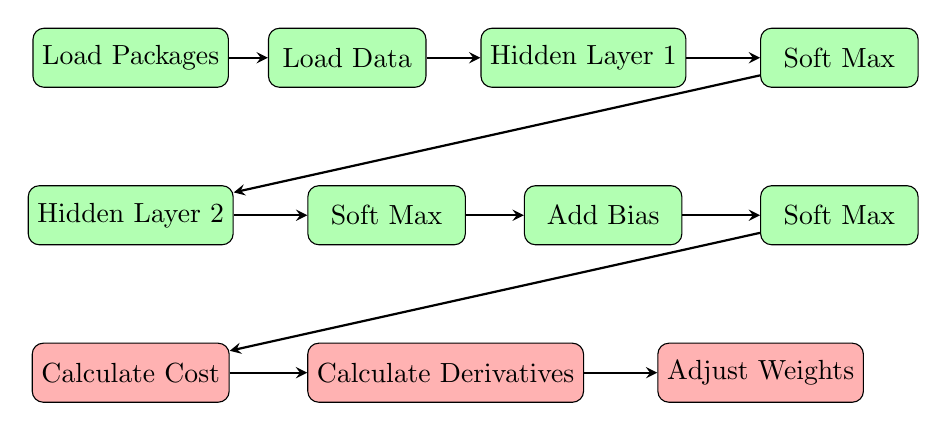
\begin{tikzpicture}[node distance=2cm]
    % Define block styles
    \tikzstyle{startstop} = [rectangle, rounded corners, minimum width=2cm, minimum height=0.75cm,text centered, draw=black, fill=red!30]
    \tikzstyle{middle} = [rectangle, rounded corners, minimum width=2cm, minimum height=0.75cm,text centered, draw=black, fill=green!30]
    \tikzstyle{arrow} = [thick, ->, >=stealth]
    \tikzstyle{noarrow} = [thick]


    % Draw nodes
    \node (start) [middle] {Load Packages};
    \node (input) [middle] at (2.75,0) {Load Data};
    \node (input2) [middle] at (5.75,0) {Hidden Layer 1};
    \node (input3) [middle] at (9,0) {Soft Max};
    \node (input4) [middle] at (0,-2) {Hidden Layer 2};
    \node (input5) [middle] at (3.25,-2) {Soft Max};
    \node (input6) [middle] at (6,-2) {Add Bias};
    \node (input7) [middle] at (9,-2) {Soft Max};
    \node (input8) [startstop] at (0,-4) {Calculate Cost};
    \node (input9) [startstop] at (4,-4) {Calculate Derivatives};
    \node (input10) [startstop] at (8,-4) {Adjust Weights};
    
    % Draw edges
    \draw [arrow] (start) -- (input);
    \draw [arrow] (input) -- (input2);
    \draw [arrow] (input2) -- (input3);
    \draw [arrow] (input3) -- (input4);
    \draw [arrow] (input4) -- (input5);
    \draw [arrow] (input5) -- (input6);
    \draw [arrow] (input6) -- (input7);
    \draw [arrow] (input7) -- (input8);
    \draw [arrow] (input8) -- (input9);
    \draw [arrow] (input9) -- (input10);
    
\end{tikzpicture}
}

\end{document}

